\chapter{\label{method}Experiments and Analysis}
\section{With Iron}
\begin{figure}[h!]
	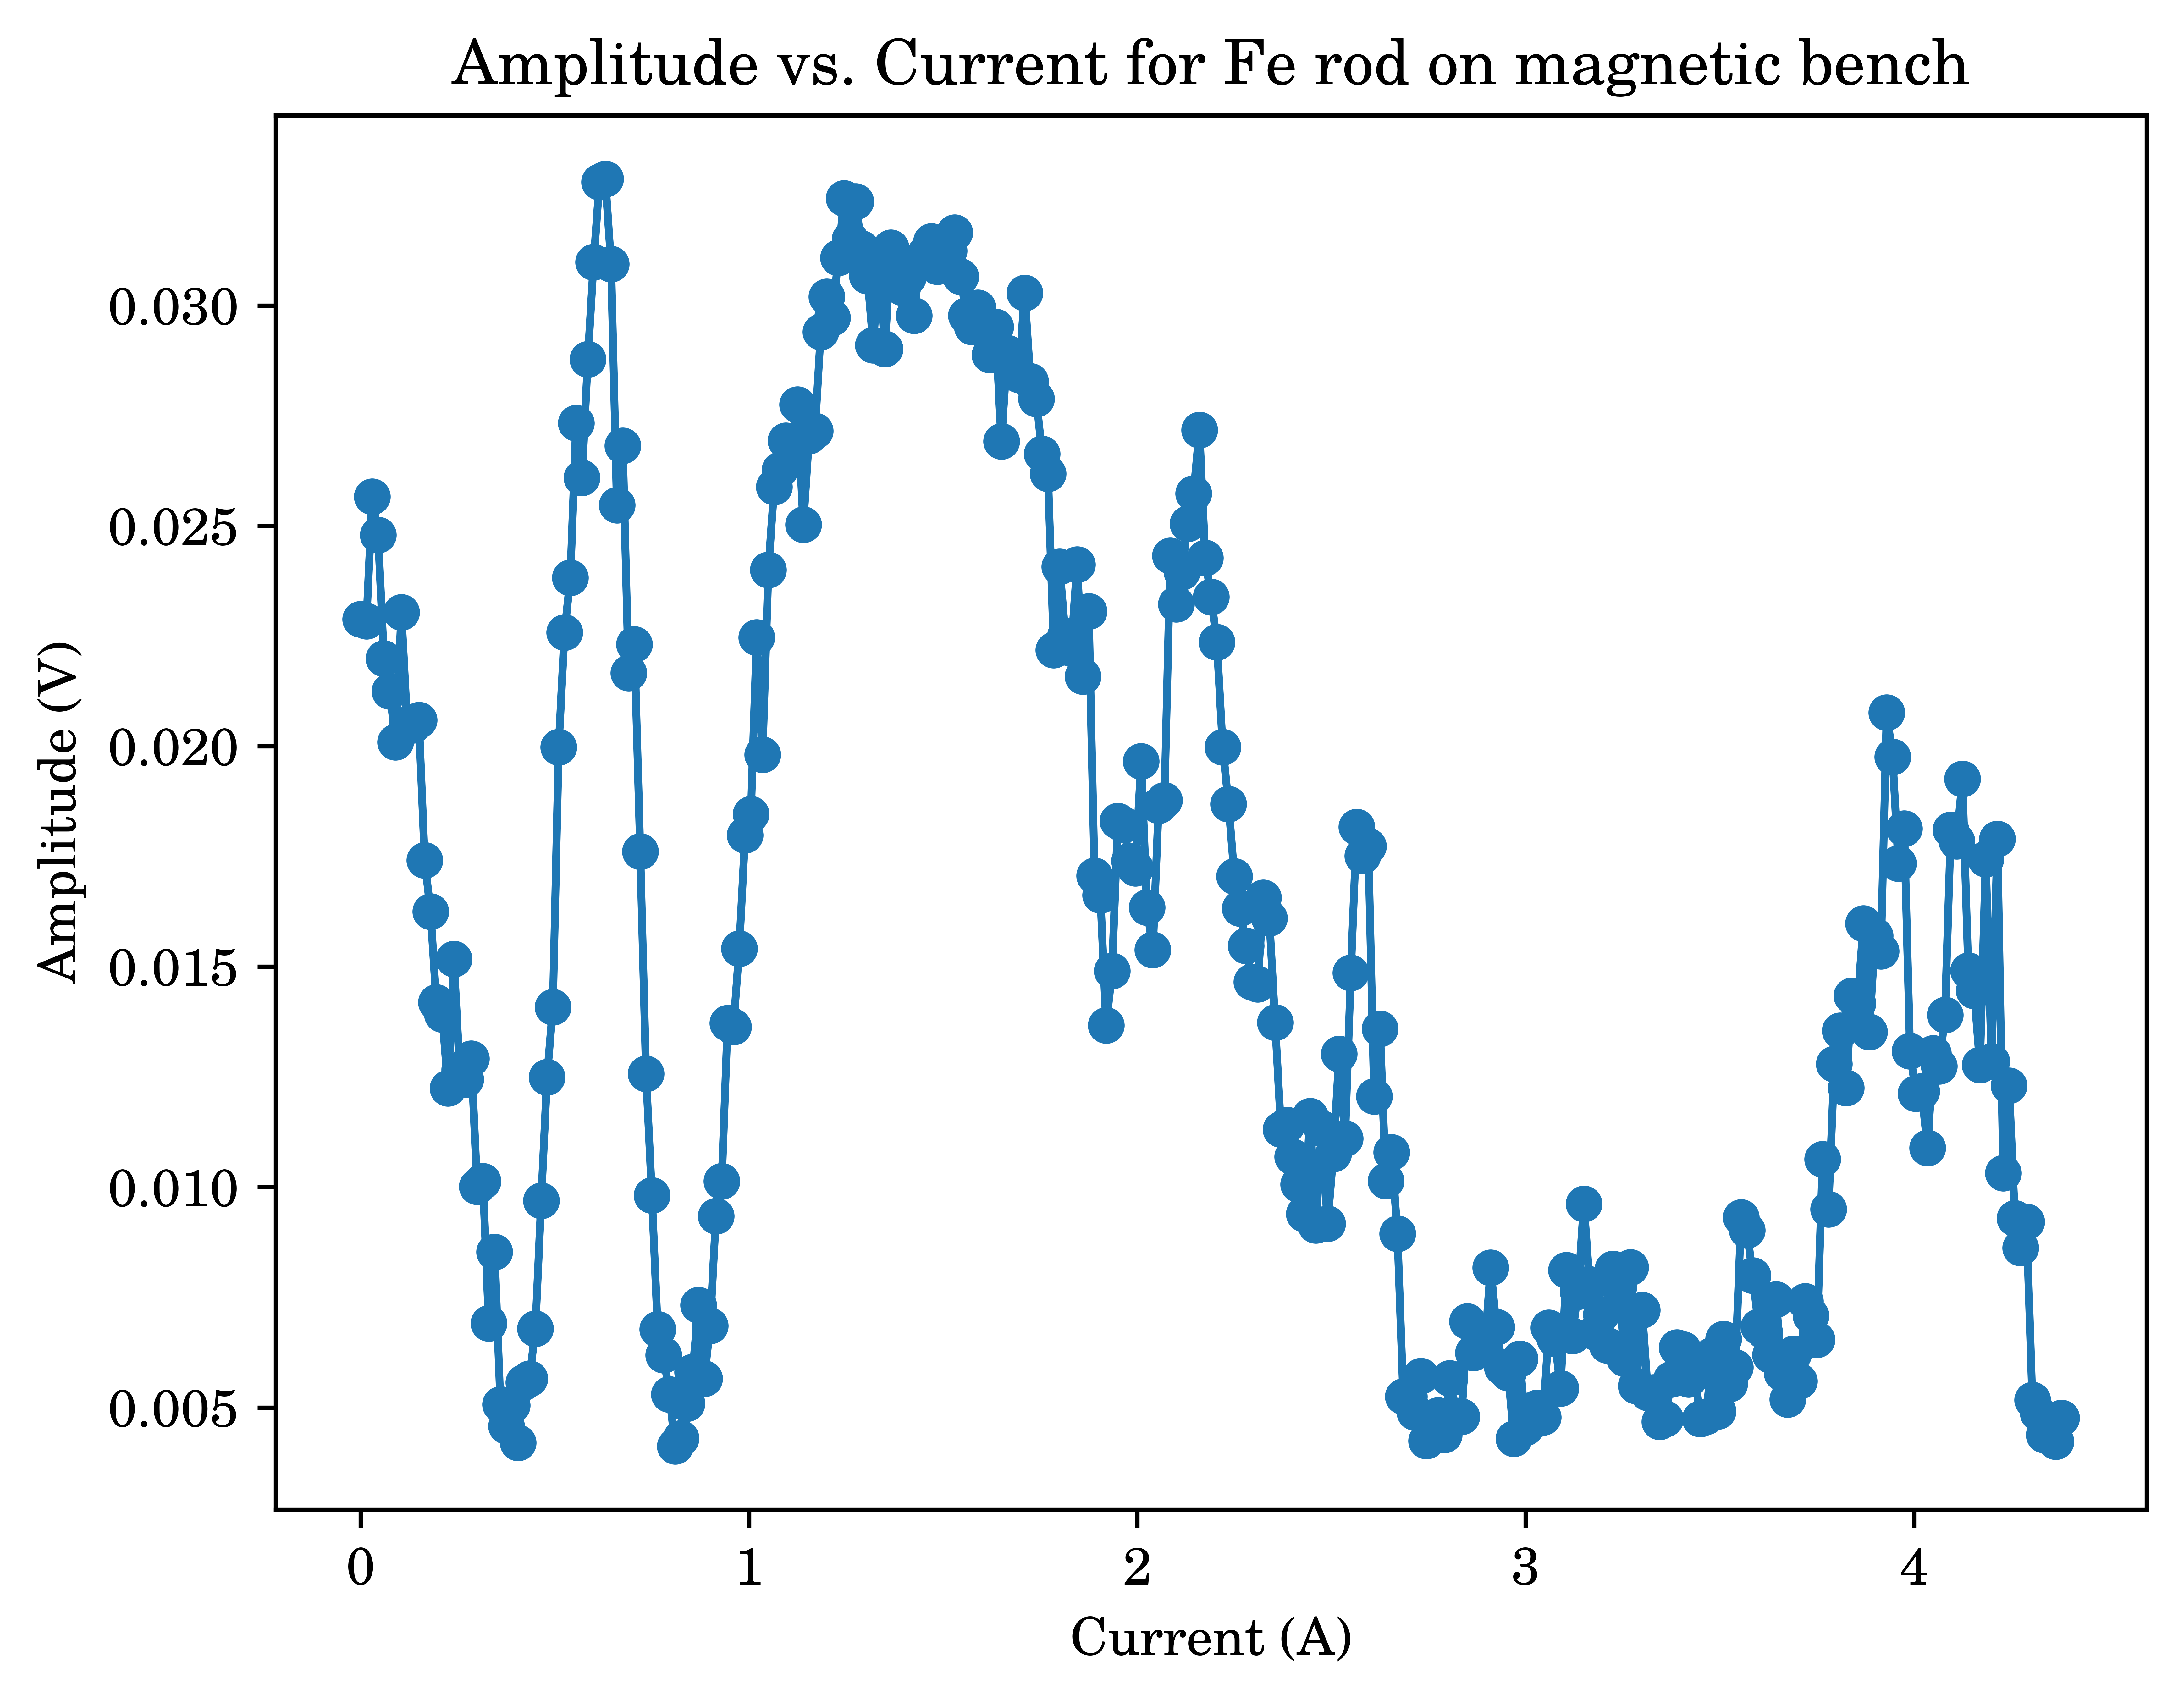
\includegraphics{data/mb-Fe-0}
	\caption{The amplitude versus current data obtained for Fe rod on the magnetic bench.}
	\label{fig:mb-fe-0}
\end{figure}
% Please add the following required packages to your document preamble:
% \usepackage{booktabs}
\begin{table}[h!]
	\centering
	\resizebox{\textwidth}{!}{%
		\begin{tabular}{@{}ccccc@{}}
			\toprule
			\textbf{\begin{tabular}[c]{@{}c@{}}Current\\ (\si{\ampere})\end{tabular}} & \textbf{\begin{tabular}[c]{@{}c@{}}Ring changes\\ ($n$)\end{tabular}} & \textbf{\begin{tabular}[c]{@{}c@{}}$\Delta l$\\ ($\times 10^{-9} \si{\meter}$)\end{tabular}} & \textbf{\begin{tabular}[c]{@{}c@{}}Magnetization, $H$\\ ($\si{\ampere \per \meter}$)\end{tabular}} & \textbf{\begin{tabular}[c]{@{}c@{}}$\Delta l/l$\\ ($\times 10^{-9} \si{\meter}$)\end{tabular}} \\ \midrule
			0.555                                                                 & 1                                                                   & 1.58E-07                                                                                & 4.66E+03                                                   & 1.11E-06                                                                                  \\
			0.57                                                                  & 1.5                                                                 & 2.37E-07                                                                                & 4.78E+03                                                   & 1.66E-06                                                                                  \\
			0.63                                                                  & 2                                                                   & 3.16E-07                                                                                & 5.29E+03                                                   & 2.21E-06                                                                                  \\
			0.66                                                                  & 1.5                                                                 & 2.37E-07                                                                                & 5.54E+03                                                   & 1.66E-06                                                                                  \\
			0.675                                                                 & 1                                                                   & 1.58E-07                                                                                & 5.66E+03                                                   & 1.11E-06                                                                                  \\
			0.69                                                                  & 0.5                                                                 & 7.91E-08                                                                                & 5.79E+03                                                   & 5.53E-07                                                                                  \\
			0.705                                                                 & 0                                                                   & 0.00E+00                                                                                & 5.92E+03                                                   & 0.00E+00                                                                                  \\ \bottomrule
		\end{tabular}
	}
	\caption{The variation in strain with applied magnetic field for Fe on the magnetic bench.}
	\label{tab:mb-Fe}
\end{table}
\begin{figure}
	\centering
	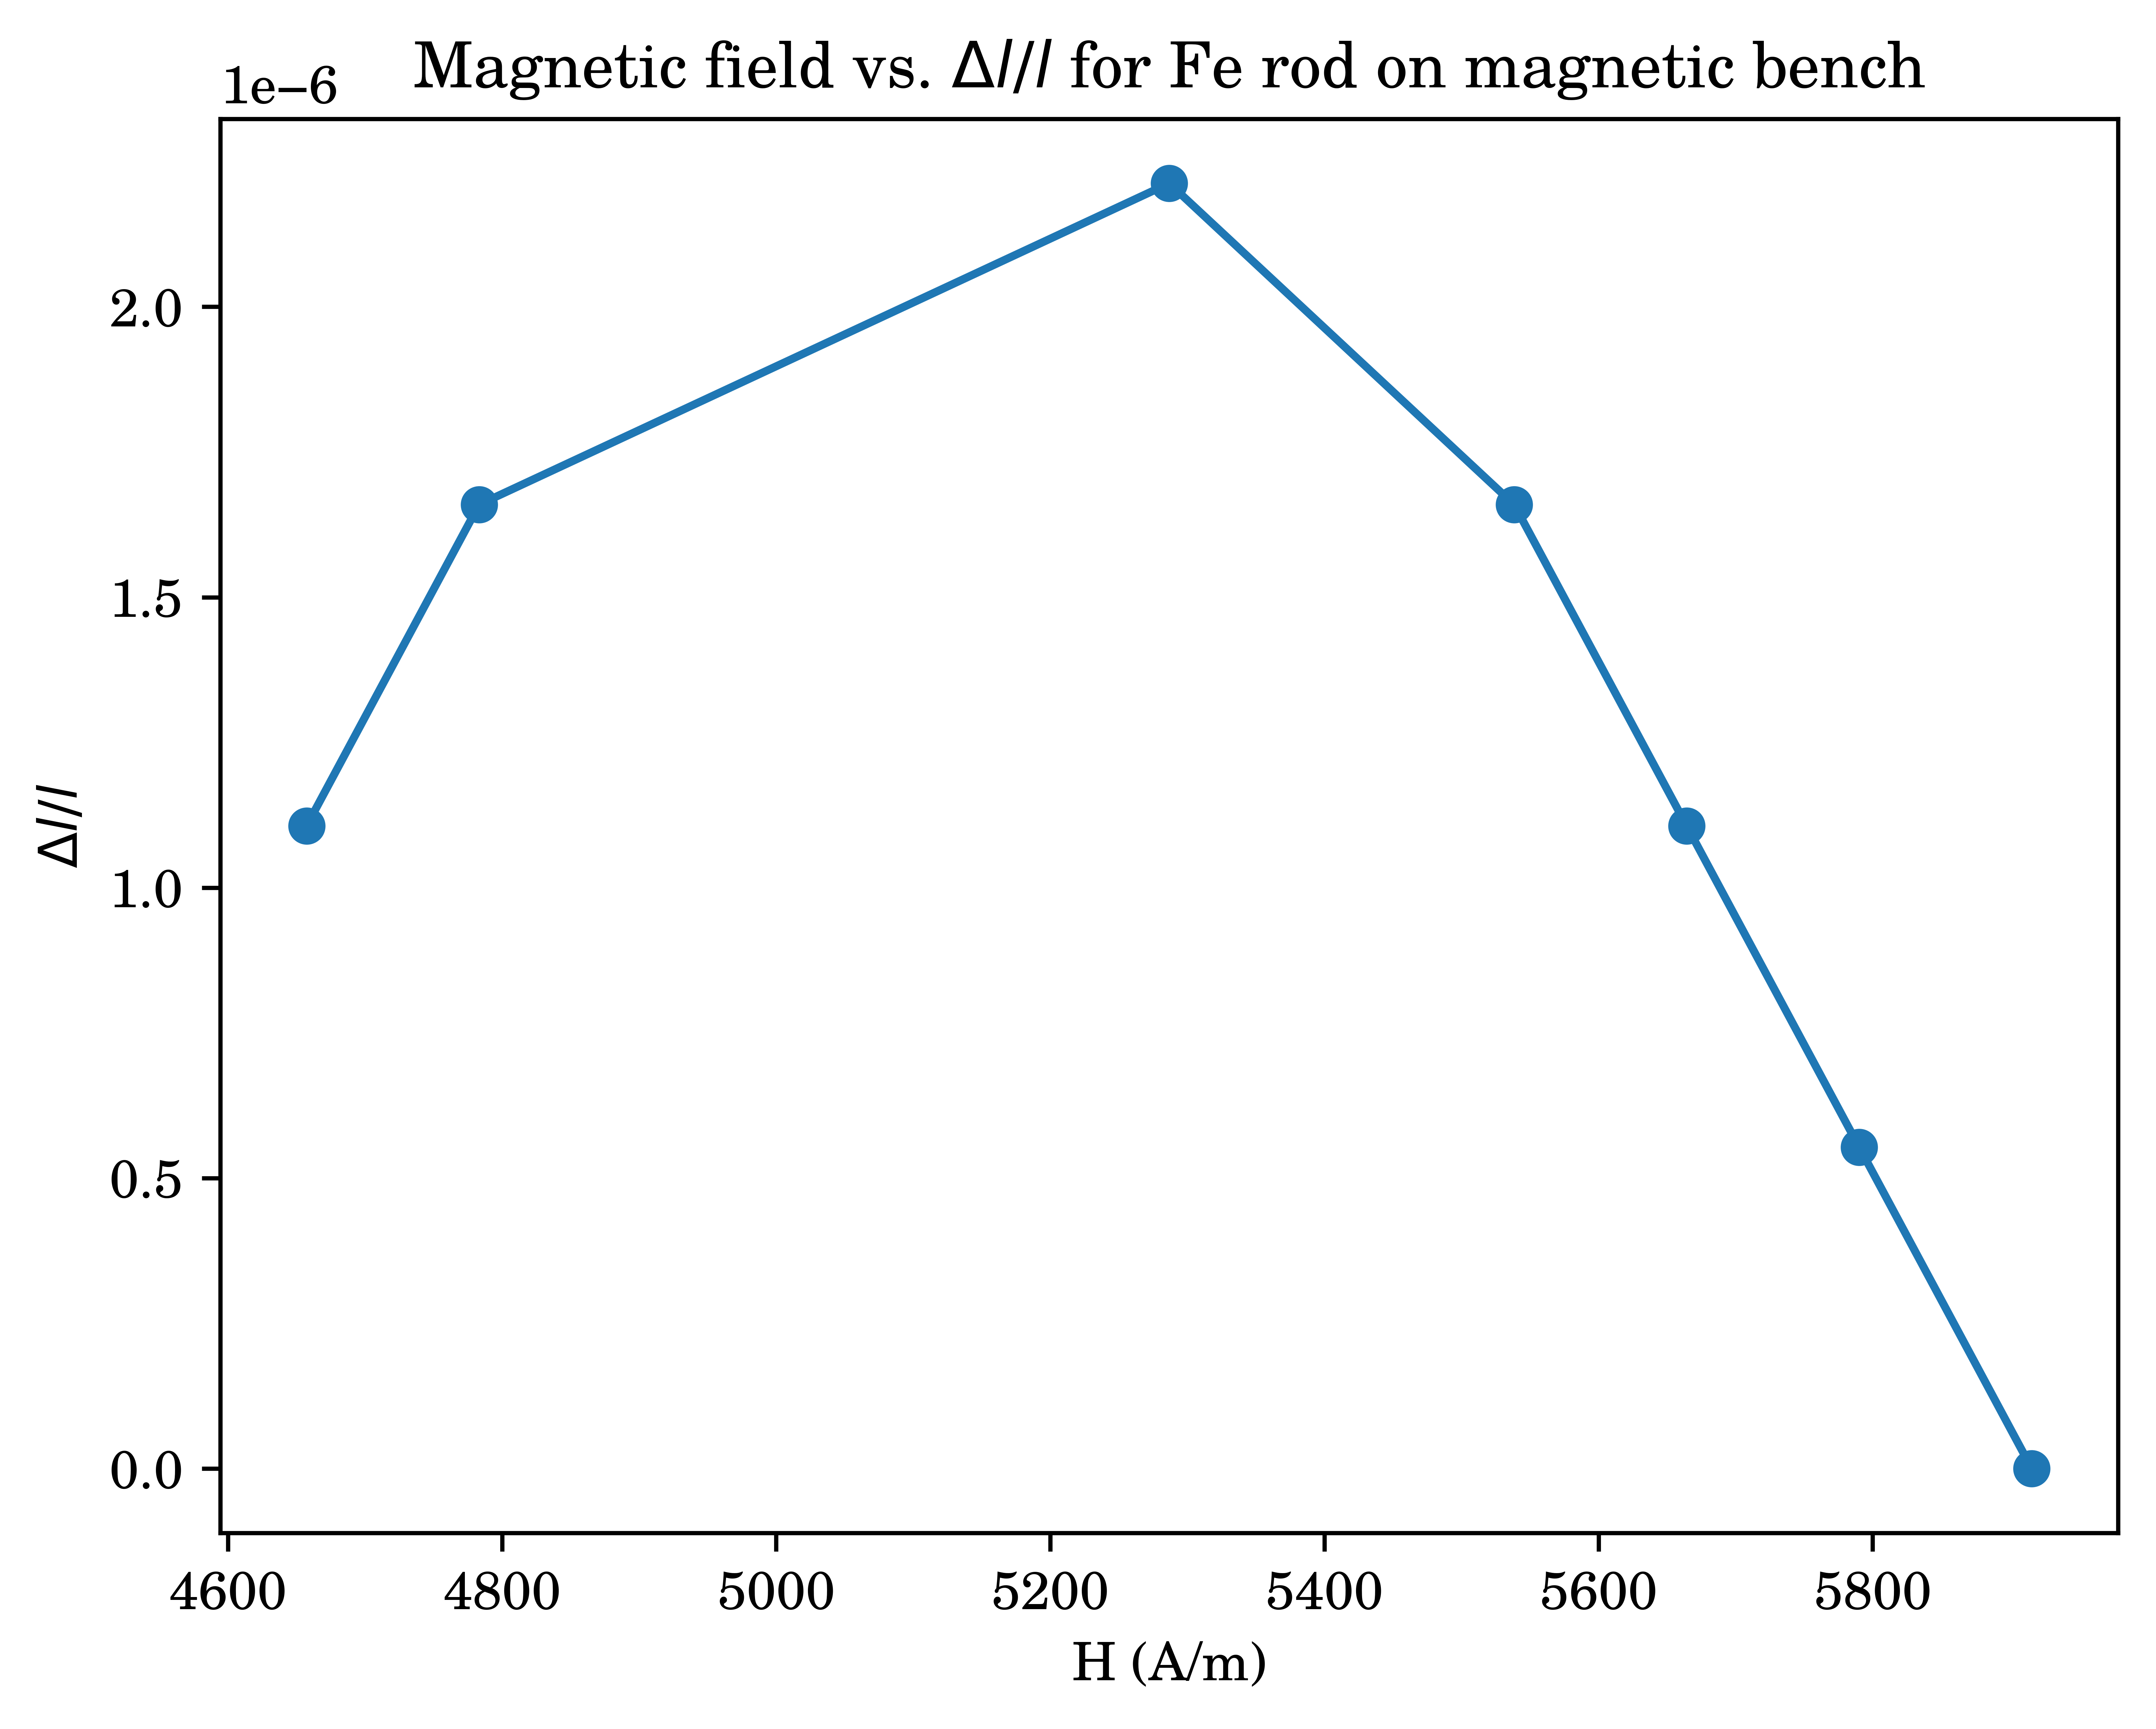
\includegraphics{data/mb-Fe-1}
	\caption{The variation in strain with applied magnetic field for Fe on the magnetic bench.}
	\label{fig:mb-fe-1}
\end{figure}

\section{With Nickel}
\begin{figure}[h!]
	\centering
	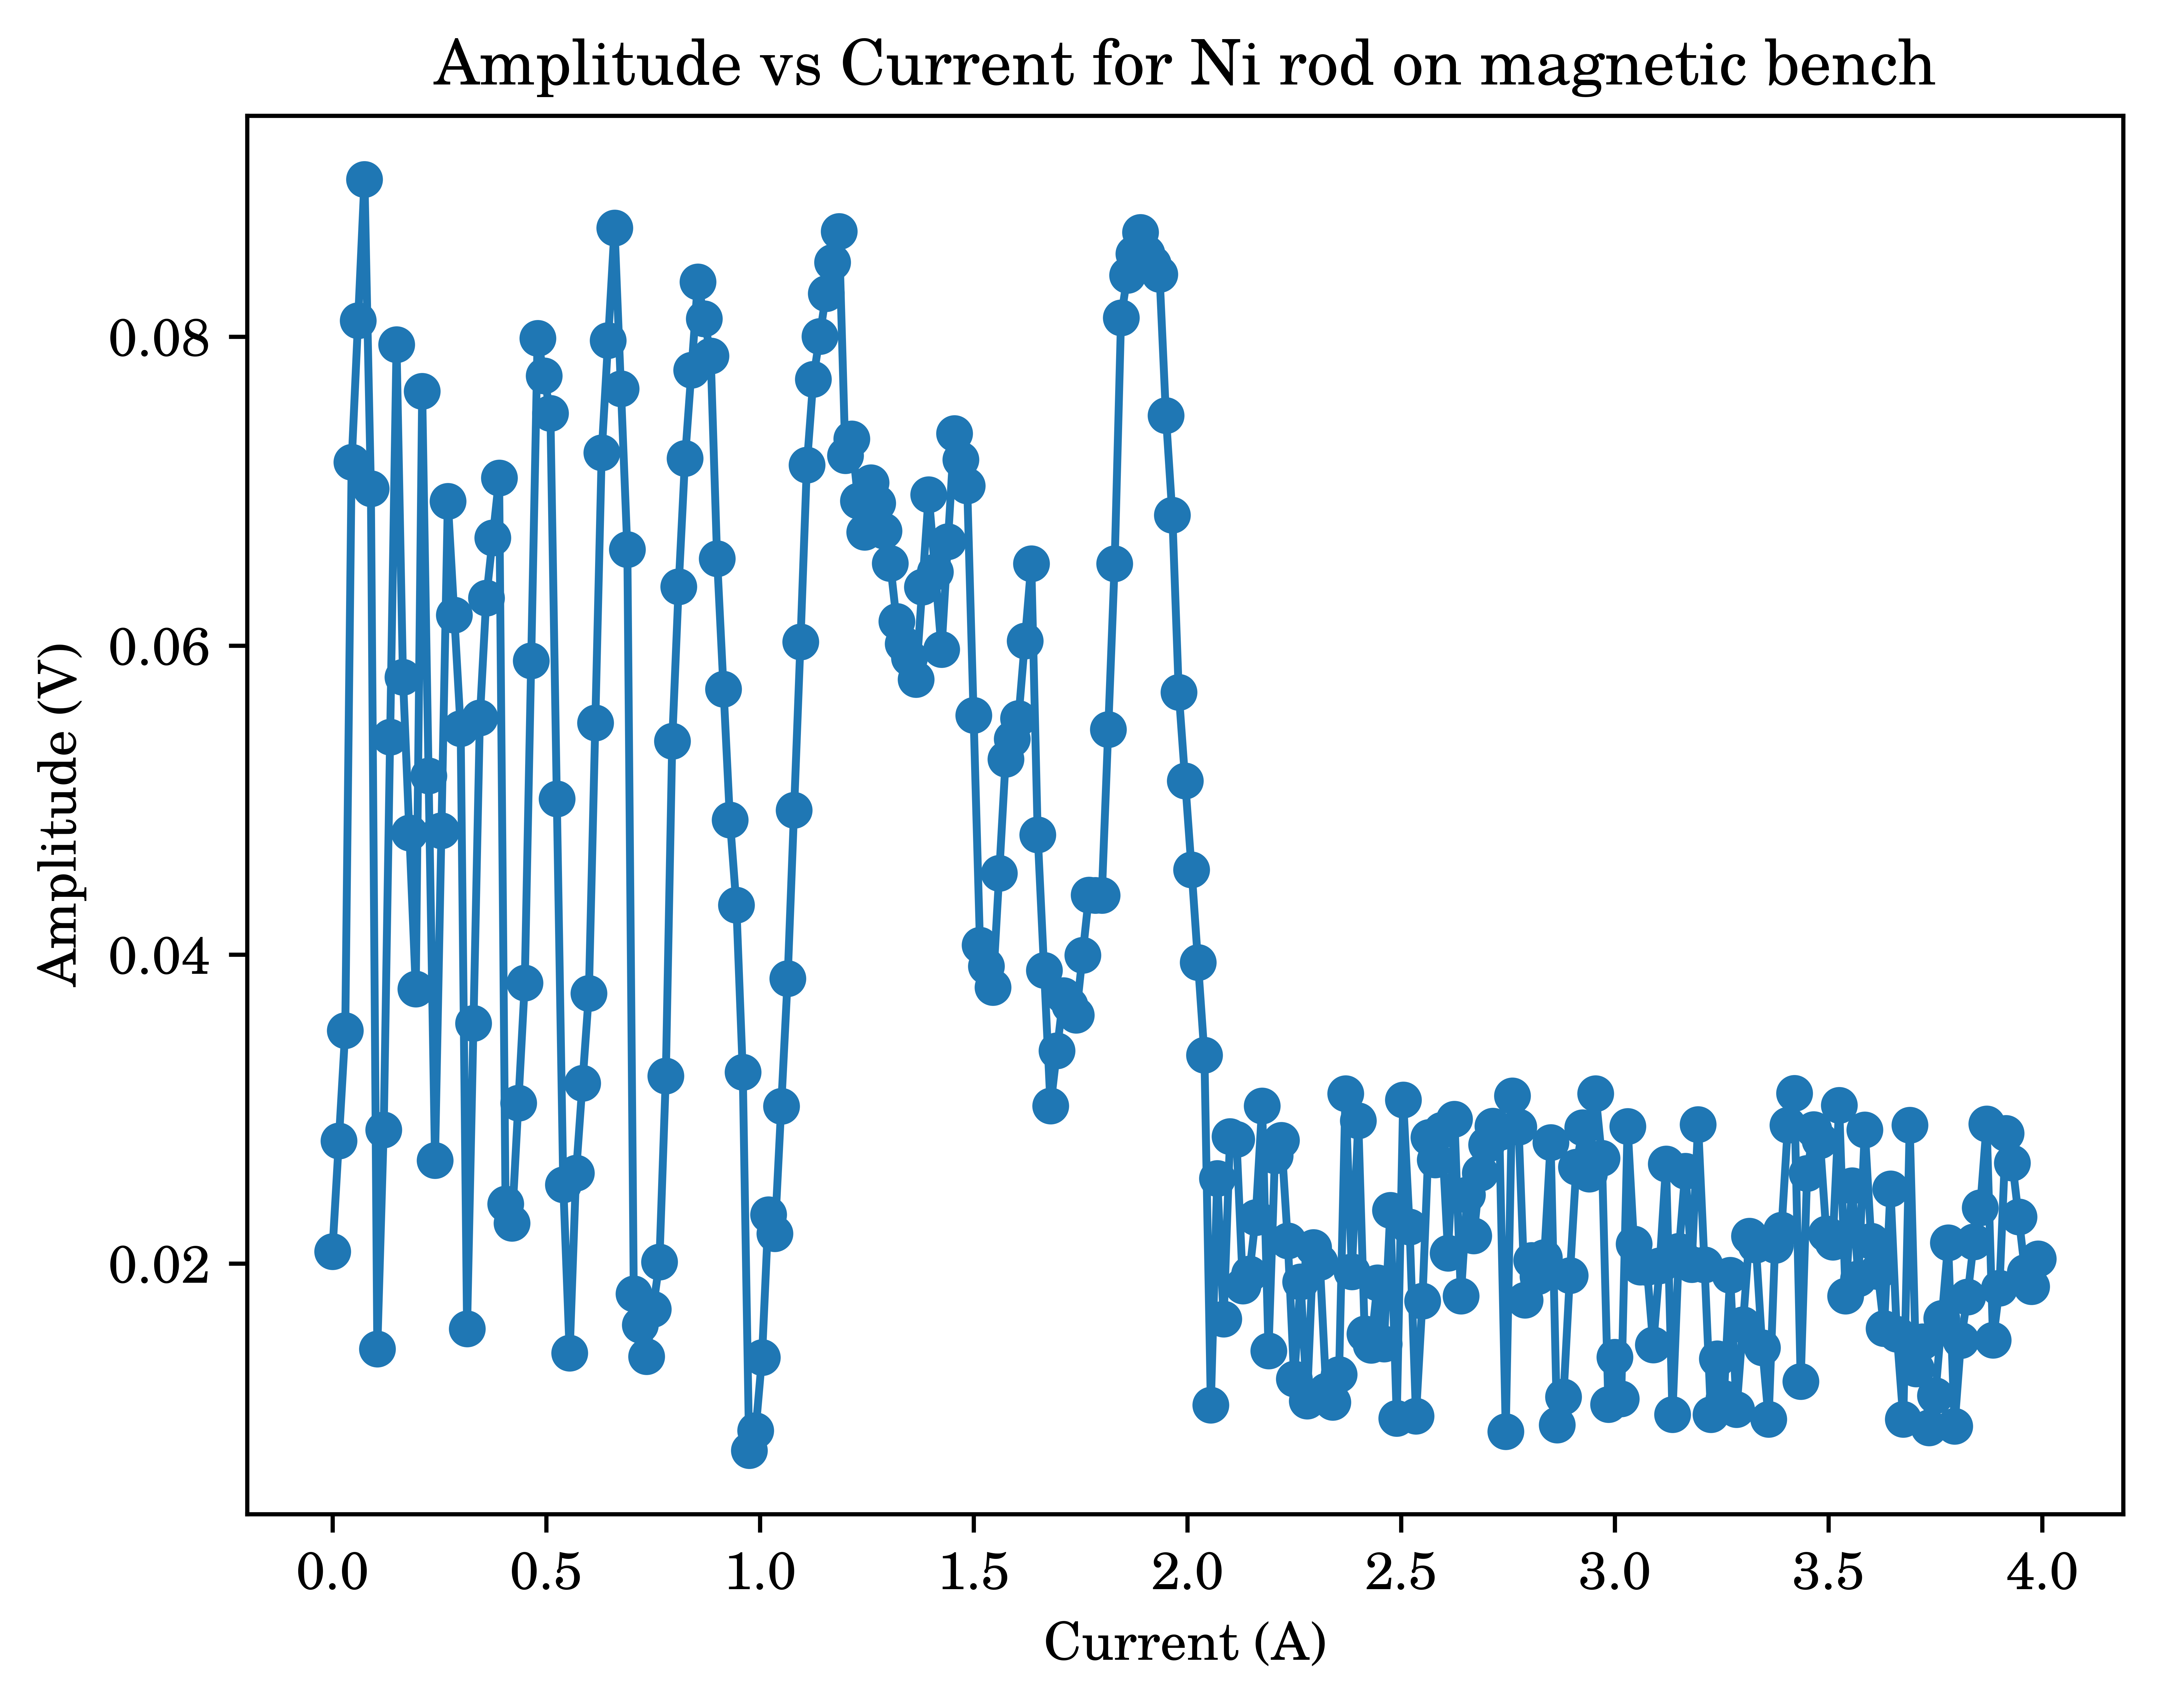
\includegraphics{data/mb-Ni-0}
	\caption{The amplitude versus current data obtained for Ni rod on the magnetic bench.}
	\label{fig:mb-ni-0}
\end{figure}

% Please add the following required packages to your document preamble:
% \usepackage{booktabs}
% \usepackage{graphicx}
\begin{table}[h!]
	\centering
	\resizebox{\textwidth}{!}{%
		\begin{tabular}{@{}ccccc@{}}
			\toprule
			\textbf{\begin{tabular}[c]{@{}c@{}}Current\\ (\si{\ampere})\end{tabular}} & \textbf{\begin{tabular}[c]{@{}c@{}}Ring changes\\ ($n$)\end{tabular}} & \textbf{\begin{tabular}[c]{@{}c@{}}$\Delta l$\\ ($\times 10^{-9} \si{\meter}$)\end{tabular}} & \textbf{\begin{tabular}[c]{@{}c@{}}Magnetization, $H$\\ ($\si{\ampere \per \meter}$)\end{tabular}} & \textbf{\begin{tabular}[c]{@{}c@{}}$\Delta l/l$\\ ($\times 10^{-9} \si{\meter}$)\end{tabular}} \\ \midrule
			0.075 & 0.5 & -7.91E-08 & 6.29E+02 & -5.53E-07 \\
			0.105 & 1   & -1.58E-07 & 8.81E+02 & -1.11E-06 \\
			0.15  & 1.5 & -2.37E-07 & 1.26E+03 & -1.66E-06 \\
			0.195 & 2   & -3.16E-07 & 1.64E+03 & -2.21E-06 \\
			0.21  & 2.5 & -3.96E-07 & 1.76E+03 & -2.77E-06 \\
			0.24  & 3   & -4.75E-07 & 2.01E+03 & -3.32E-06 \\
			0.27  & 3.5 & -5.54E-07 & 2.27E+03 & -3.87E-06 \\
			0.315 & 4   & -6.33E-07 & 2.64E+03 & -4.43E-06 \\
			0.39  & 4.5 & -7.12E-07 & 3.27E+03 & -4.98E-06 \\
			0.42  & 5   & -7.91E-07 & 3.52E+03 & -5.53E-06 \\
			0.48  & 5.5 & -8.70E-07 & 4.03E+03 & -6.08E-06 \\
			0.555 & 6   & -9.49E-07 & 4.66E+03 & -6.64E-06 \\
			0.66  & 6.5 & -1.03E-06 & 5.54E+03 & -7.19E-06 \\
			0.735 & 7   & -1.11E-06 & 6.17E+03 & -7.74E-06 \\
			0.855 & 7.5 & -1.19E-06 & 7.17E+03 & -8.30E-06 \\
			0.975 & 8   & -1.27E-06 & 8.18E+03 & -8.85E-06 \\
			1.02  & 8.5 & -1.34E-06 & 8.56E+03 & -9.40E-06 \\
			1.035 & 9   & -1.42E-06 & 8.69E+03 & -9.96E-06 \\
			1.185 & 9.5 & -1.50E-06 & 9.94E+03 & -1.05E-05 \\ \bottomrule
		\end{tabular}%
	}
	\caption{The variation in strain with applied magnetic field for Ni on the magnetic bench.}
	\label{tab:my-table}
\end{table}
\begin{figure}
	\centering
	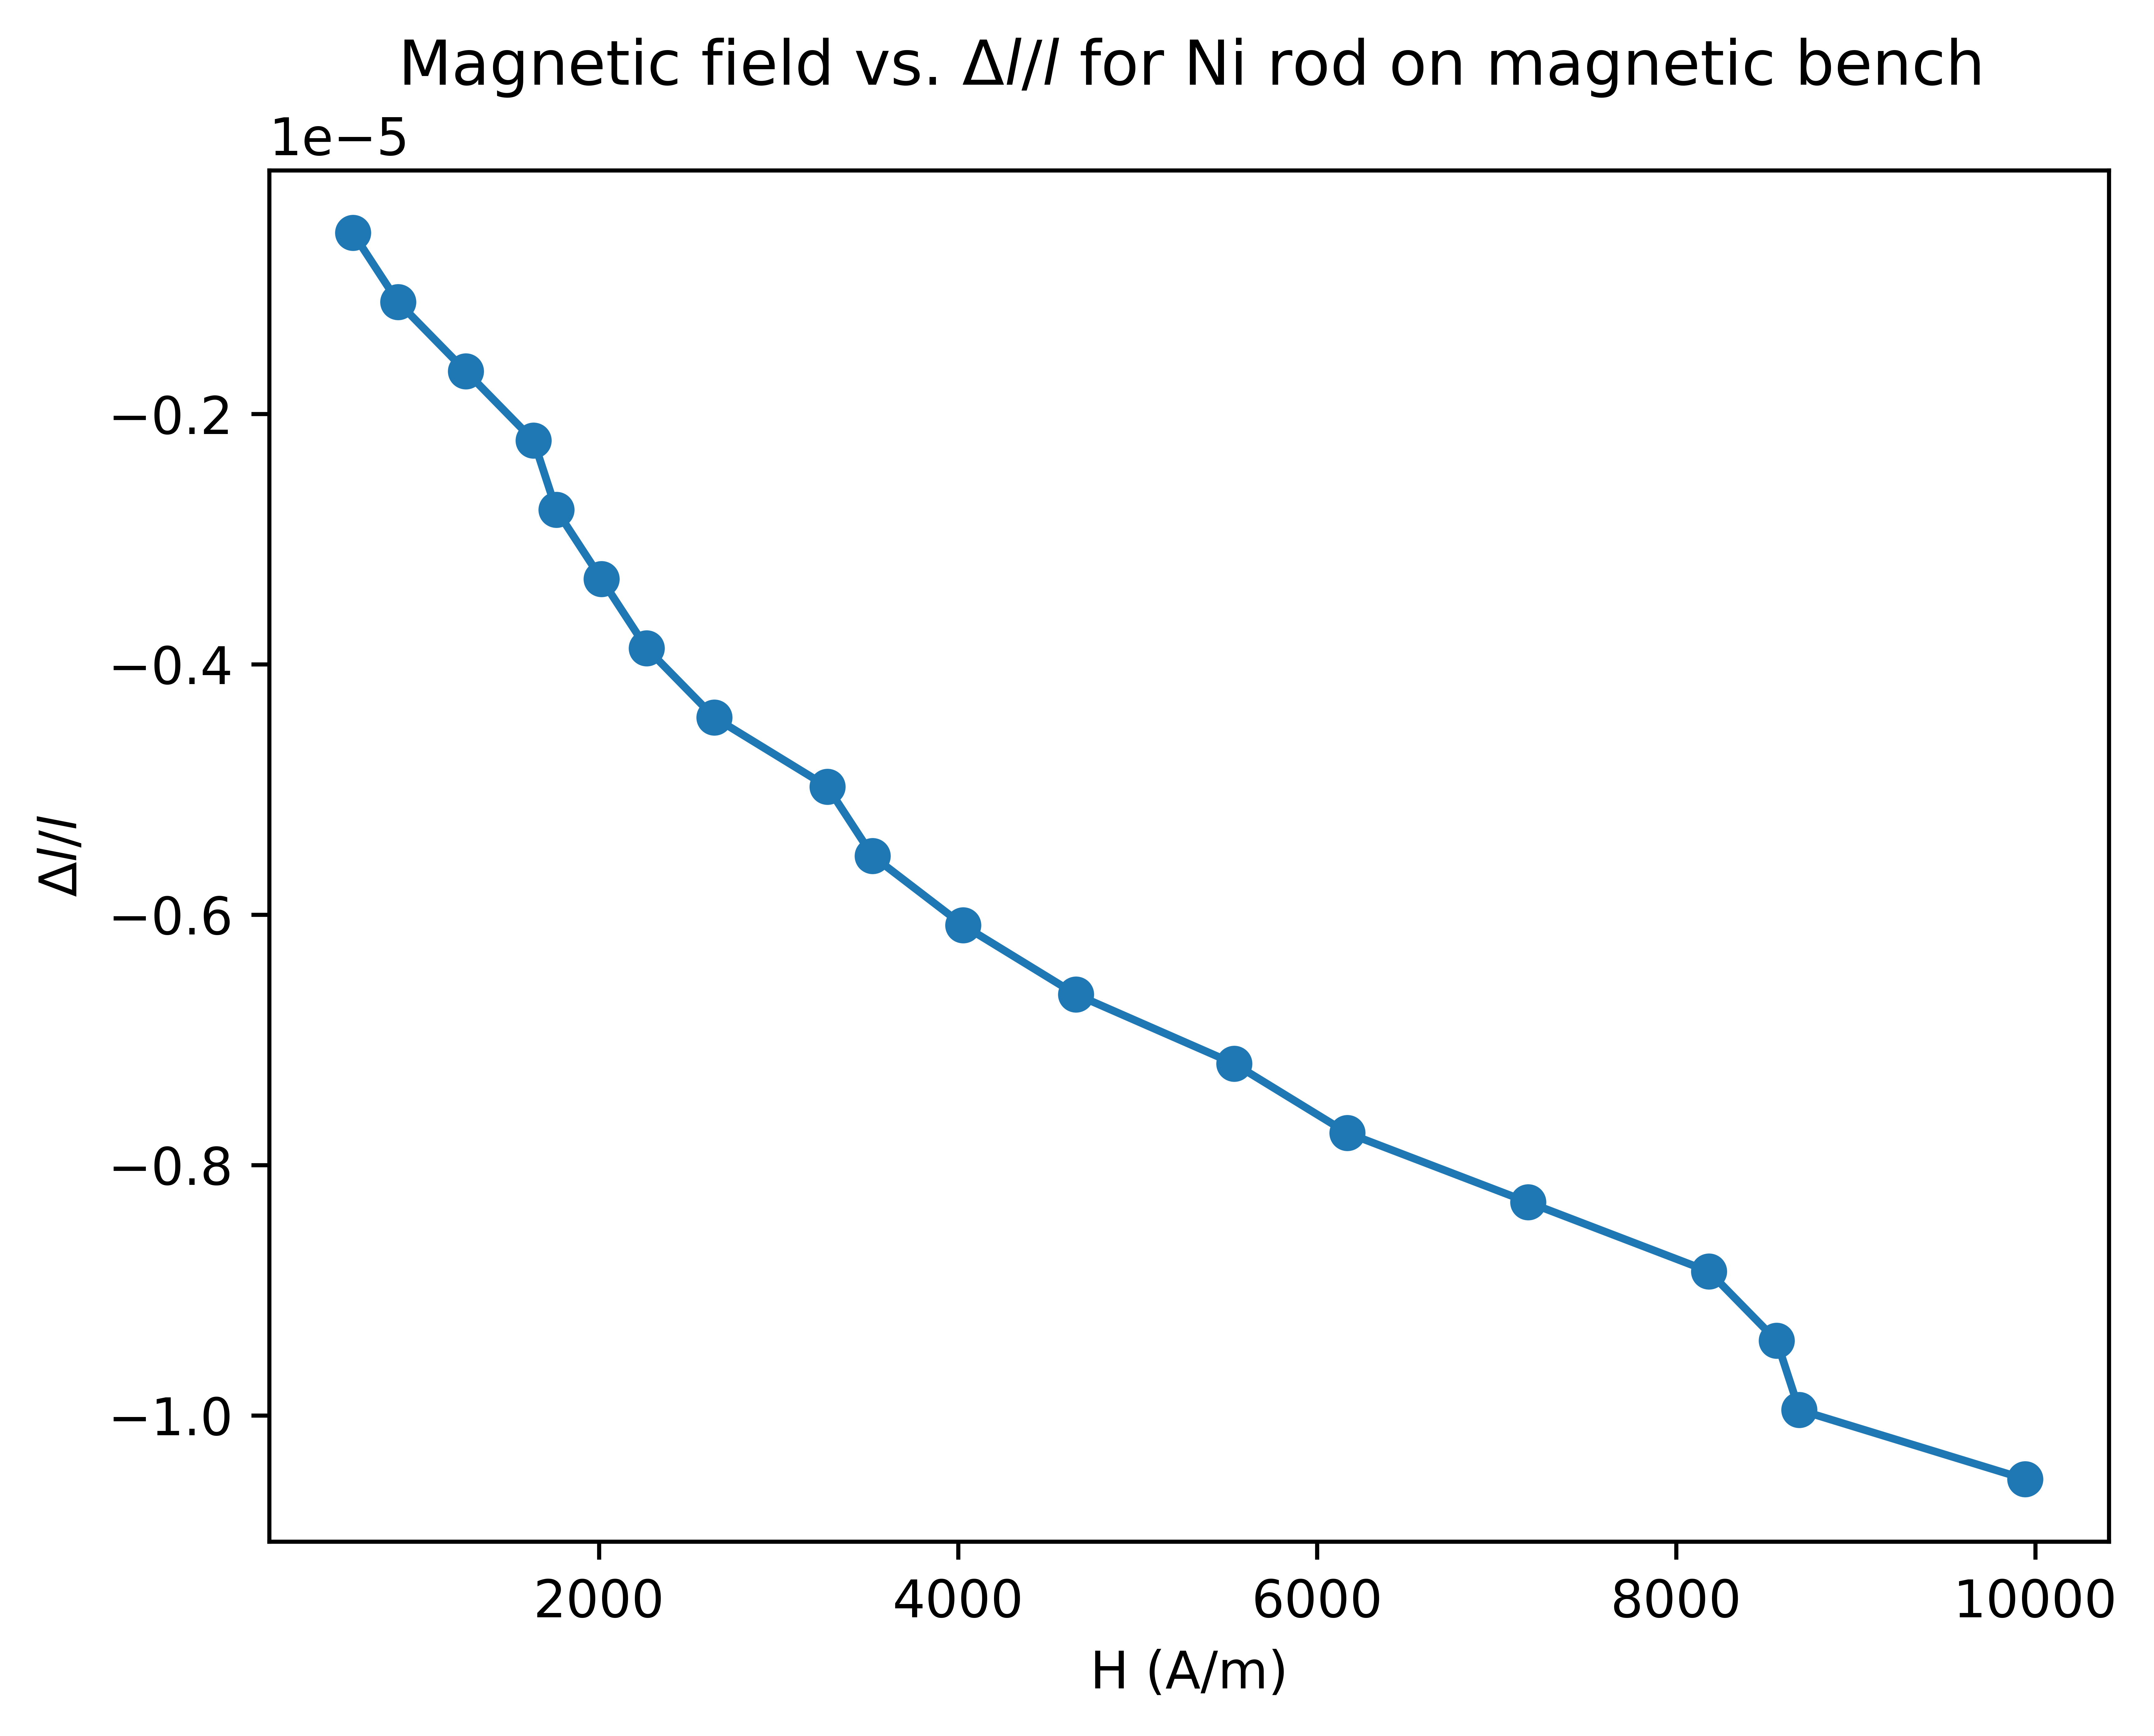
\includegraphics{data/mb-Ni-1}
	\caption{The variation in strain with applied magnetic field for Ni on the magnetic bench.}
	\label{fig:mb-ni-1}
\end{figure}

\section{With Copper}
\begin{figure}
	\centering
	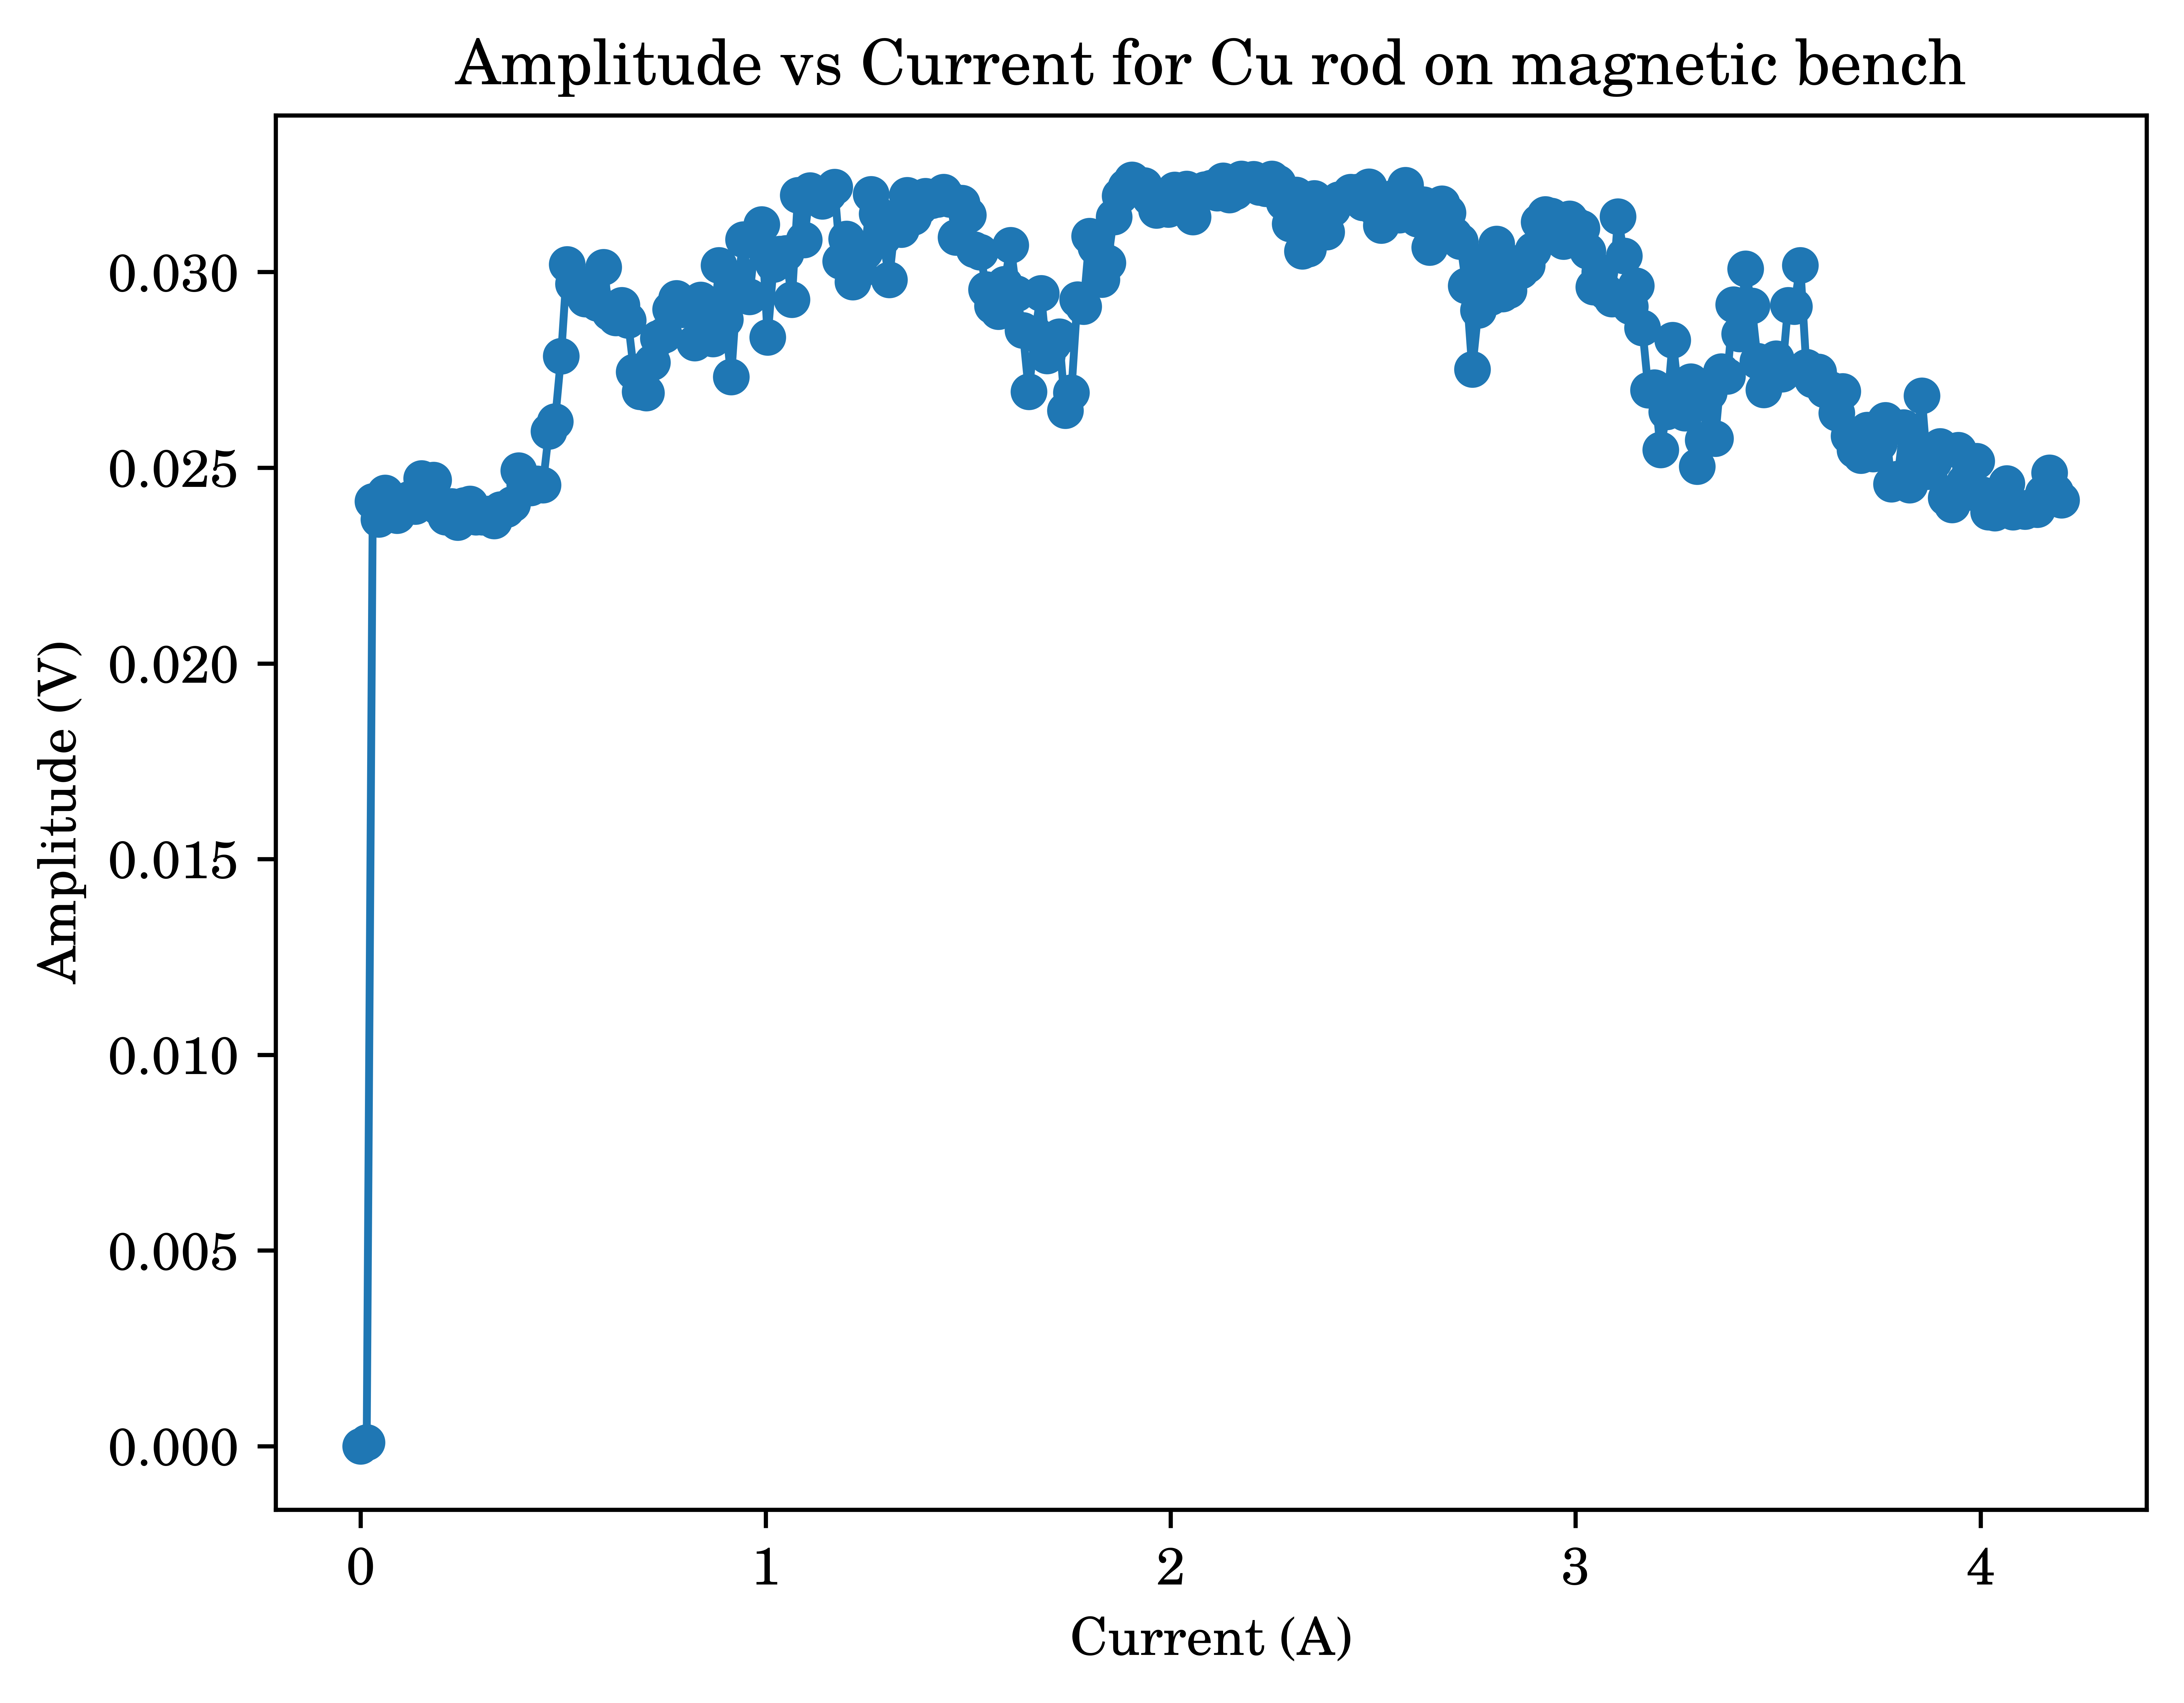
\includegraphics{data/mb-Cu-0}
	\caption{The amplitude versus current data obtained for Cu rod on the magnetic bench.}
	\label{fig:mb-cu-0}
\end{figure}

\setcounter{equation}{0}
\setcounter{table}{0}
\setcounter{figure}{0}
%\baselineskip 24pt
